\chapter{Cahaya dan Bayang-bayang}\label{ch:g1:light-and-shadows}

Matikan lampu di ruangan tanpa jendela: semuanya lenyap. Nyalakan
lagi: ruangan itu kembali. Melihat memerlukan \omterm{def:g1:light-and-shadows:source}{cahaya}. Dan di mana ada
\omterm{def:g1:light-and-shadows:source}{cahaya}, di situ ada \omterm{def:g1:light-and-shadows:shadow}{bayang-bayang} --- kembaran gelapmu yang setia
mengikutimu di setiap trotoar yang terkena matahari. Mari kita cari
tahu dari mana \omterm{def:g1:light-and-shadows:source}{cahaya} datang, dan bagaimana \omterm{def:g1:light-and-shadows:shadow}{bayang-bayang} terbentuk.

\section{Dari mana cahaya datang}

\begin{definition}[Sumber cahaya]\label{def:g1:light-and-shadows:source}
Sebuah \emph{sumber cahaya}\index{sumber cahaya} adalah benda yang
membuat \emph{cahaya}\index{cahaya} sendiri: Matahari, lampu, nyala
lilin, kunang-kunang. Benda lain --- buku, bola, dinding, dirimu ---
tidak membuat cahaya sendiri: kita hanya melihat benda-benda itu
ketika cahaya dari sebuah sumber jatuh padanya.
\end{definition}

\begin{example}[Sumber atau bukan?]\label{ex:g1:light-and-shadows:sources}
Matahari, senter, korek api yang menyala, dan layar televisi semuanya
membuat \omterm{def:g1:light-and-shadows:source}{cahaya}: itulah sumber. Bulan, cermin, dan dinding putih bisa
tampak sangat terang, tetapi tidak membuat \omterm{def:g1:light-and-shadows:source}{cahaya} sendiri ---
benda-benda itu hanya memantulkan kembali \omterm{def:g1:light-and-shadows:source}{cahaya} yang sampai padanya.
Matikan lampunya, dan cermin yang paling terang pun menjadi gelap.
\end{example}

\begin{example}[Cobalah: ruangan gelap]\label{ex:g1:light-and-shadows:darkroom}
Pada malam hari, tutuplah daun jendela atau tirai sebuah ruangan,
matikan semua lampu, dan tunggulah sambil menghitung pelan sampai
$20$. Apa yang kamu lihat? Mula-mula hampir tidak ada apa-apa ---
tanpa sumber, tidak ada \omterm{def:g1:light-and-shadows:source}{cahaya} untuk melihat. Lalu bukalah pintunya
sedikit: satu iris \omterm{def:g1:light-and-shadows:source}{cahaya} yang tipis sudah cukup untuk mengembalikan
meja, kursi, dan mainan.
\end{example}

\begin{remark}[Jangan pernah menatap Matahari]\label{rem:g1:light-and-shadows:sun}
Matahari adalah \omterm{def:g1:light-and-shadows:source}{sumber cahaya} terkuat yang pernah kita temui. Jangan
pernah menatapnya langsung, walau sekejap, apalagi lewat teropong atau
kaca pembesar: \omterm{def:g1:light-and-shadows:source}{cahayanya} begitu kuat sehingga dapat merusak matamu
untuk selamanya. Matahari dinikmati dari samping --- lewat \omterm{def:g1:light-and-shadows:source}{cahaya} yang
ia lemparkan ke segala benda lain.
\end{remark}

\section{Bagaimana bayang-bayang terbentuk}

\begin{definition}[Bayang-bayang]\label{def:g1:light-and-shadows:shadow}
Sebuah \emph{bayang-bayang}\index{bayang-bayang} adalah daerah gelap
yang muncul di belakang benda yang menghalangi \omterm{def:g1:light-and-shadows:source}{cahaya}. \omterm{def:g1:light-and-shadows:source}{Cahaya} tidak
dapat menembus tubuhmu, sehingga di belakangmu tanah tidak menerima
\omterm{def:g1:light-and-shadows:source}{cahaya} Matahari: daerah gelap berbentuk dirimu itulah bayang-bayangmu.
\end{definition}

\begin{omfigure}
\begin{tikzpicture}[scale=0.85]
  % two rays from the lamp, exactly tangent to the ball (computed:
  % source (0,1.5), ball center (4.2,1.5), r=0.55 -> wall hits y=1.5±1.004)
  \draw[omThm] (0,1.5) -- (7.6,2.504);
  \draw[omThm] (0,1.5) -- (7.6,0.496);
  % free rays that miss the ball entirely
  \draw[omThm] (0,1.5) ++(32:0.42) -- ++(32:2.4);
  \draw[omThm] (0,1.5) ++(-32:0.42) -- ++(-32:2.4);
  \fill[omThm] (0,1.5) circle (0.3);
  \draw[thick, fill=omDef, fill opacity=0.3] (4.2,1.5) circle (0.55);
  \draw[very thick] (7.6,-0.4) -- (7.6,3.4);
  \draw[line width=3.5pt, omExo] (7.6,0.496) -- (7.6,2.504);
  \node[below, font=\small] at (0,1.0) {lampu};
  \node[below, font=\small] at (4.2,0.7) {bola};
  \node[right, font=\small] at (7.75,1.5) {bayang-bayang};
  \node[right, font=\small] at (7.75,3.0) {dinding};
\end{tikzpicture}

{\small Lampu menyinari, bola menghalangi, dinding di belakangnya
tetap gelap: lampu, penghalang, \omterm{def:g1:light-and-shadows:shadow}{bayang-bayang} --- selalu berurutan
begitu, pada satu garis lurus.}
\end{omfigure}

\begin{method}[Membuat bayang-bayang yang tajam]\label{met:g1:light-and-shadows:make}
\begin{enumerate}
  \item Gelapkan ruangan --- \omterm{def:g1:light-and-shadows:shadow}{bayang-bayang} bersembunyi kalau \omterm{def:g1:light-and-shadows:source}{cahaya}
        datang dari mana-mana;
  \item nyalakan \emph{satu} lampu atau senter;
  \item pegang sebuah mainan di antara lampu dan dinding;
  \item lihatlah dinding: di situ ada \omterm{def:g1:light-and-shadows:shadow}{bayang-bayangnya}, di sisi mainan
        yang jauh dari lampu.
\end{enumerate}
Dekatkan mainan itu ke lampu: \omterm{def:g1:light-and-shadows:shadow}{bayang-bayangnya} membesar. Dekatkan ke
dinding: \omterm{def:g1:light-and-shadows:shadow}{bayang-bayangnya} menyusut sampai sebesar mainannya sendiri.
\end{method}

\begin{example}[Cobalah: bayang-bayang binatang]\label{ex:g1:light-and-shadows:animals}
Dengan lampu pada \cref{met:g1:light-and-shadows:make}, taruhlah
tanganmu di dalam \omterm{def:g1:light-and-shadows:source}{cahaya}, bukan mainan: dua jari tegak menjadi telinga
kelinci, dua ibu jari bersilang menjadi burung terbang. Dinding
menampilkan bentuk yang digunting tanganmu dari \omterm{def:g1:light-and-shadows:source}{cahaya} ---
\omterm{def:g1:light-and-shadows:shadow}{bayang-bayang} selalu menyimpan bentuk penghalangnya, dilihat dari
lampu.
\end{example}

\begin{remark}[Bayang-bayang bukan benda]\label{rem:g1:light-and-shadows:notathing}
Kamu tidak bisa memungut \omterm{def:g1:light-and-shadows:shadow}{bayang-bayang}, melipatnya, atau menyimpannya
di dalam kotak. \omterm{def:g1:light-and-shadows:shadow}{Bayang-bayang} tidak terbuat dari apa pun: ia adalah
\emph{tempat yang kehilangan \omterm{def:g1:light-and-shadows:source}{cahaya}}. Itulah sebabnya ia lenyap
seketika saat lampu padam --- tidak ada apa pun di sana yang bisa
tertinggal.
\end{remark}

\section{Bayang-bayang mengikuti cahaya}

\begin{example}[Bayang-bayang ada di sisi mana?]\label{ex:g1:light-and-shadows:opposite}
Pada pagi hari, Matahari berada di satu sisimu dan bayang-bayangmu
terbaring di sisi \emph{yang lain}. Hadapkan wajahmu ke Matahari:
bayang-bayangmu bersembunyi di belakangmu. Balikkan punggungmu ke
Matahari: bayang-bayangmu memanjang di depan. \omterm{def:g1:light-and-shadows:shadow}{Bayang-bayang} selalu
berada tepat berseberangan dengan sumbernya.
\end{example}

\begin{omfigure}
\begin{tikzpicture}[scale=0.75]
  % low sun: the ray from the Sun grazing the stick's tip is drawn
  % straight; the shadow ends exactly where that ray meets the ground
  % (sun (0.7,2.2), tip (3.4,1.2) -> ground at x=6.64)
  \fill[omThm] (0.7,2.2) circle (0.4);
  \foreach \a in {0,45,...,315} {
    \draw[omThm] (0.7,2.2) ++(\a:0.55) -- ++(\a:0.25);
  }
  \draw[omThm] (0.7,2.2) -- (6.64,0);
  \draw[line width=2.6pt] (3.4,0) -- (3.4,1.2);
  \draw[thick] (2.2,0) -- (7.0,0);
  \draw[line width=3.5pt, omExo] (3.4,-0.09) -- (6.64,-0.09);
  \node[below, font=\small] at (4.6,-0.35) {matahari rendah: bayang-bayang panjang};
  % high sun: same stick, the grazing ray is steep
  % (sun (8.6,3.6), tip (10.2,1.2) -> ground at x=11.0)
  \fill[omThm] (8.6,3.6) circle (0.4);
  \foreach \a in {0,45,...,315} {
    \draw[omThm] (8.6,3.6) ++(\a:0.55) -- ++(\a:0.25);
  }
  \draw[omThm] (8.6,3.6) -- (11.0,0);
  \draw[line width=2.6pt] (10.2,0) -- (10.2,1.2);
  \draw[thick] (9.0,0) -- (11.8,0);
  \draw[line width=3.5pt, omExo] (10.2,-0.09) -- (11.0,-0.09);
  \node[below, font=\small] at (10.4,-0.35) {matahari tinggi: bayang-bayang pendek};
\end{tikzpicture}

{\small Tongkat yang sama, pagi dan tengah hari. \omterm{def:g1:light-and-shadows:shadow}{Bayang-bayang}
berakhir tepat di tempat sinar lurus yang menyerempet ujung tongkat
menyentuh tanah: Matahari yang rendah memanjangkannya, Matahari yang
tinggi memendekkannya.}
\end{omfigure}

\begin{omfigure}
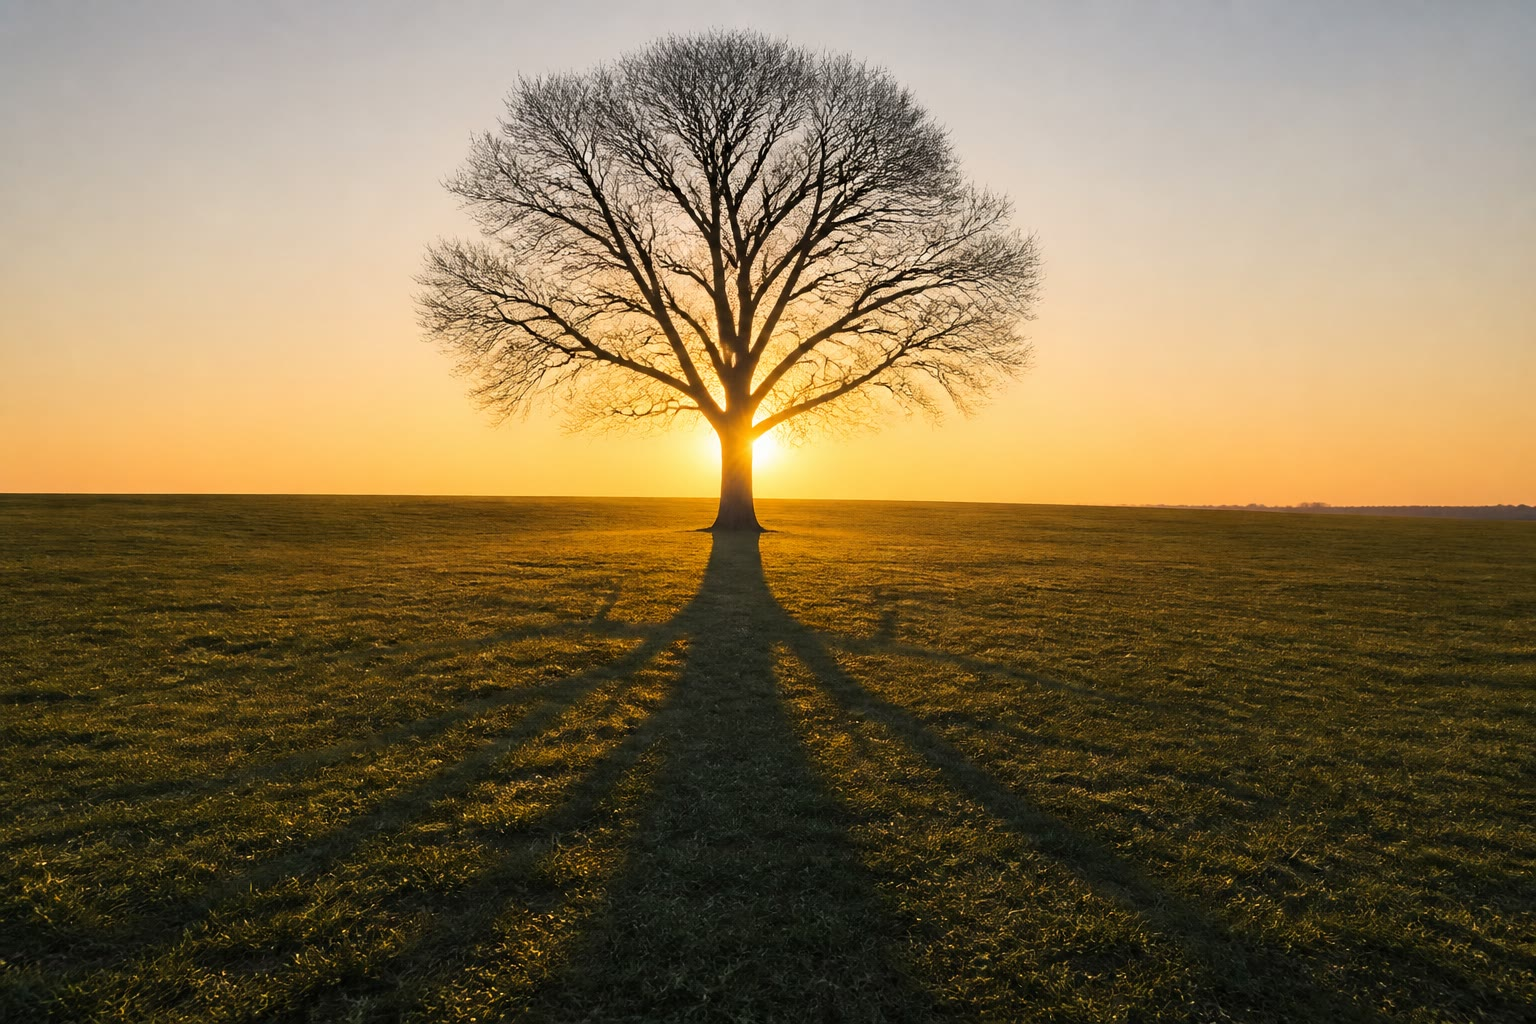
\includegraphics[width=0.6\linewidth]{images/book1/ai/g1-light-shadows-long-shadow.jpg}

{\small Matahari petang yang rendah, \omterm{def:g1:light-and-shadows:shadow}{bayang-bayang} yang panjang: makin rendah Matahari tergantung, makin jauh setiap \omterm{def:g1:light-and-shadows:shadow}{bayang-bayang} memanjang.}
\end{omfigure}

\begin{example}[Cobalah: kapur di sekeliling bayang-bayang]\label{ex:g1:light-and-shadows:chalk}
Pada pagi yang cerah, berdirilah diam di halaman bermain sementara
seorang teman menggambar garis kapur di sekeliling bayang-bayangmu.
Kembalilah sesudah makan siang dan berdirilah di tempat yang sama:
bayang-bayangmu sudah keluar dari garis kapurnya dan berubah
panjangnya! Matahari berpindah tempat di langit --- dan \omterm{def:g1:light-and-shadows:shadow}{bayang-bayang}
mengikutinya. Bab berikutnya mengikuti Matahari sepanjang harinya.
\end{example}

\section{Latihan}

\begin{exercise}[$\star$]\label{exo:g1:light-and-shadows:1}
Kelompokkan menjadi \omterm{def:g1:light-and-shadows:source}{sumber cahaya} dan bukan sumber: nyala lilin; \ Bulan;
\ kunang-kunang; \ cermin; \ senter; \ dinding putih.
\end{exercise}

\begin{exercise}[$\star$]\label{exo:g1:light-and-shadows:2}
Mengapa kamu tidak dapat melihat apa pun di ruangan tertutup tanpa
jendela dan tanpa lampu? Apa yang tidak ada di sana?
\end{exercise}

\begin{exercise}[$\star$]\label{exo:g1:light-and-shadows:3}
Sebutkan tiga hal yang diperlukan untuk membuat \omterm{def:g1:light-and-shadows:shadow}{bayang-bayang} pada
dinding, dan urutkan ketiganya pada sebuah garis.
\end{exercise}

\begin{exercise}[$\star$]\label{exo:g1:light-and-shadows:4}
Matahari berada di sebelah kirimu. Bayang-bayangmu ada di sebelah
mana? Kamu berbalik seluruhnya --- sekarang ada di mana?
\end{exercise}

\begin{exercise}[$\star$]\label{exo:g1:light-and-shadows:5}
Dengan \cref{met:g1:light-and-shadows:make}, buatlah \omterm{def:g1:light-and-shadows:shadow}{bayang-bayang}
mainan yang sama mula-mula besar sekali, lalu kecil. Apa yang kamu
pindahkan, dan ke arah mana?
\end{exercise}

\begin{exercise}[$\star$]\label{exo:g1:light-and-shadows:6}
Dapatkah \omterm{def:g1:light-and-shadows:shadow}{bayang-bayang} dipungut dan dimasukkan ke saku? Jelaskan apa
sebenarnya \omterm{def:g1:light-and-shadows:shadow}{bayang-bayang} itu, dengan \cref{rem:g1:light-and-shadows:notathing}.
\end{exercise}

\begin{exercise}[$\star$]\label{exo:g1:light-and-shadows:7}
Mengapa kamu tidak boleh menatap Matahari, padahal menatap lampu
hanya menyilaukan sedikit?
\end{exercise}

\begin{exercise}[$\star$]\label{exo:g1:light-and-shadows:8}
Pada tengah hari Matahari tergantung tinggi; pada sore hari ia
tergantung rendah. Kapan bayang-bayangmu lebih panjang? Gambarlah dua
\omterm{def:g1:light-and-shadows:shadow}{bayang-bayang} sebuah pohon, satu untuk tiap saat itu.
\end{exercise}

\begin{exercise}[$\star\star$]\label{exo:g1:light-and-shadows:9}
Mia berkata: ``Bayang-bayangku tadi ada di depanku, dan sesudah aku
berbalik ia ada di belakangku --- jadi \omterm{def:g1:light-and-shadows:shadow}{bayang-bayang} itu ikut
berbalik.'' Sam berkata \omterm{def:g1:light-and-shadows:shadow}{bayang-bayang} itu sama sekali tidak bergerak.
Ingat \cref{ex:g1:light-and-shadows:opposite}: siapa yang benar, dan
mengapa \emph{tampaknya} \omterm{def:g1:light-and-shadows:shadow}{bayang-bayang} itu ikut berbalik?
\end{exercise}
